\section{Spatial Correlation Across PJM Zones (Q8)}\label{sec:spatial}

A geographically distributed fleet only smooths forecast errors if they are spatially independent. To assess spatial independence, we measure the spatial coherence by computing (i) zone-to-zone correlation, and (ii) the distance over which site-to-site correlation decays.

\subsection{Zone-to-zone correlation}

We collapse the \num{896} sites into their nine PJM zones, form a zone-mean error series
per zone (all lead times pooled), and Pearson-correlate the nine series per variable
(Figure~\ref{fig:zonecorr}).

\begin{figure}[H]
  \centering
  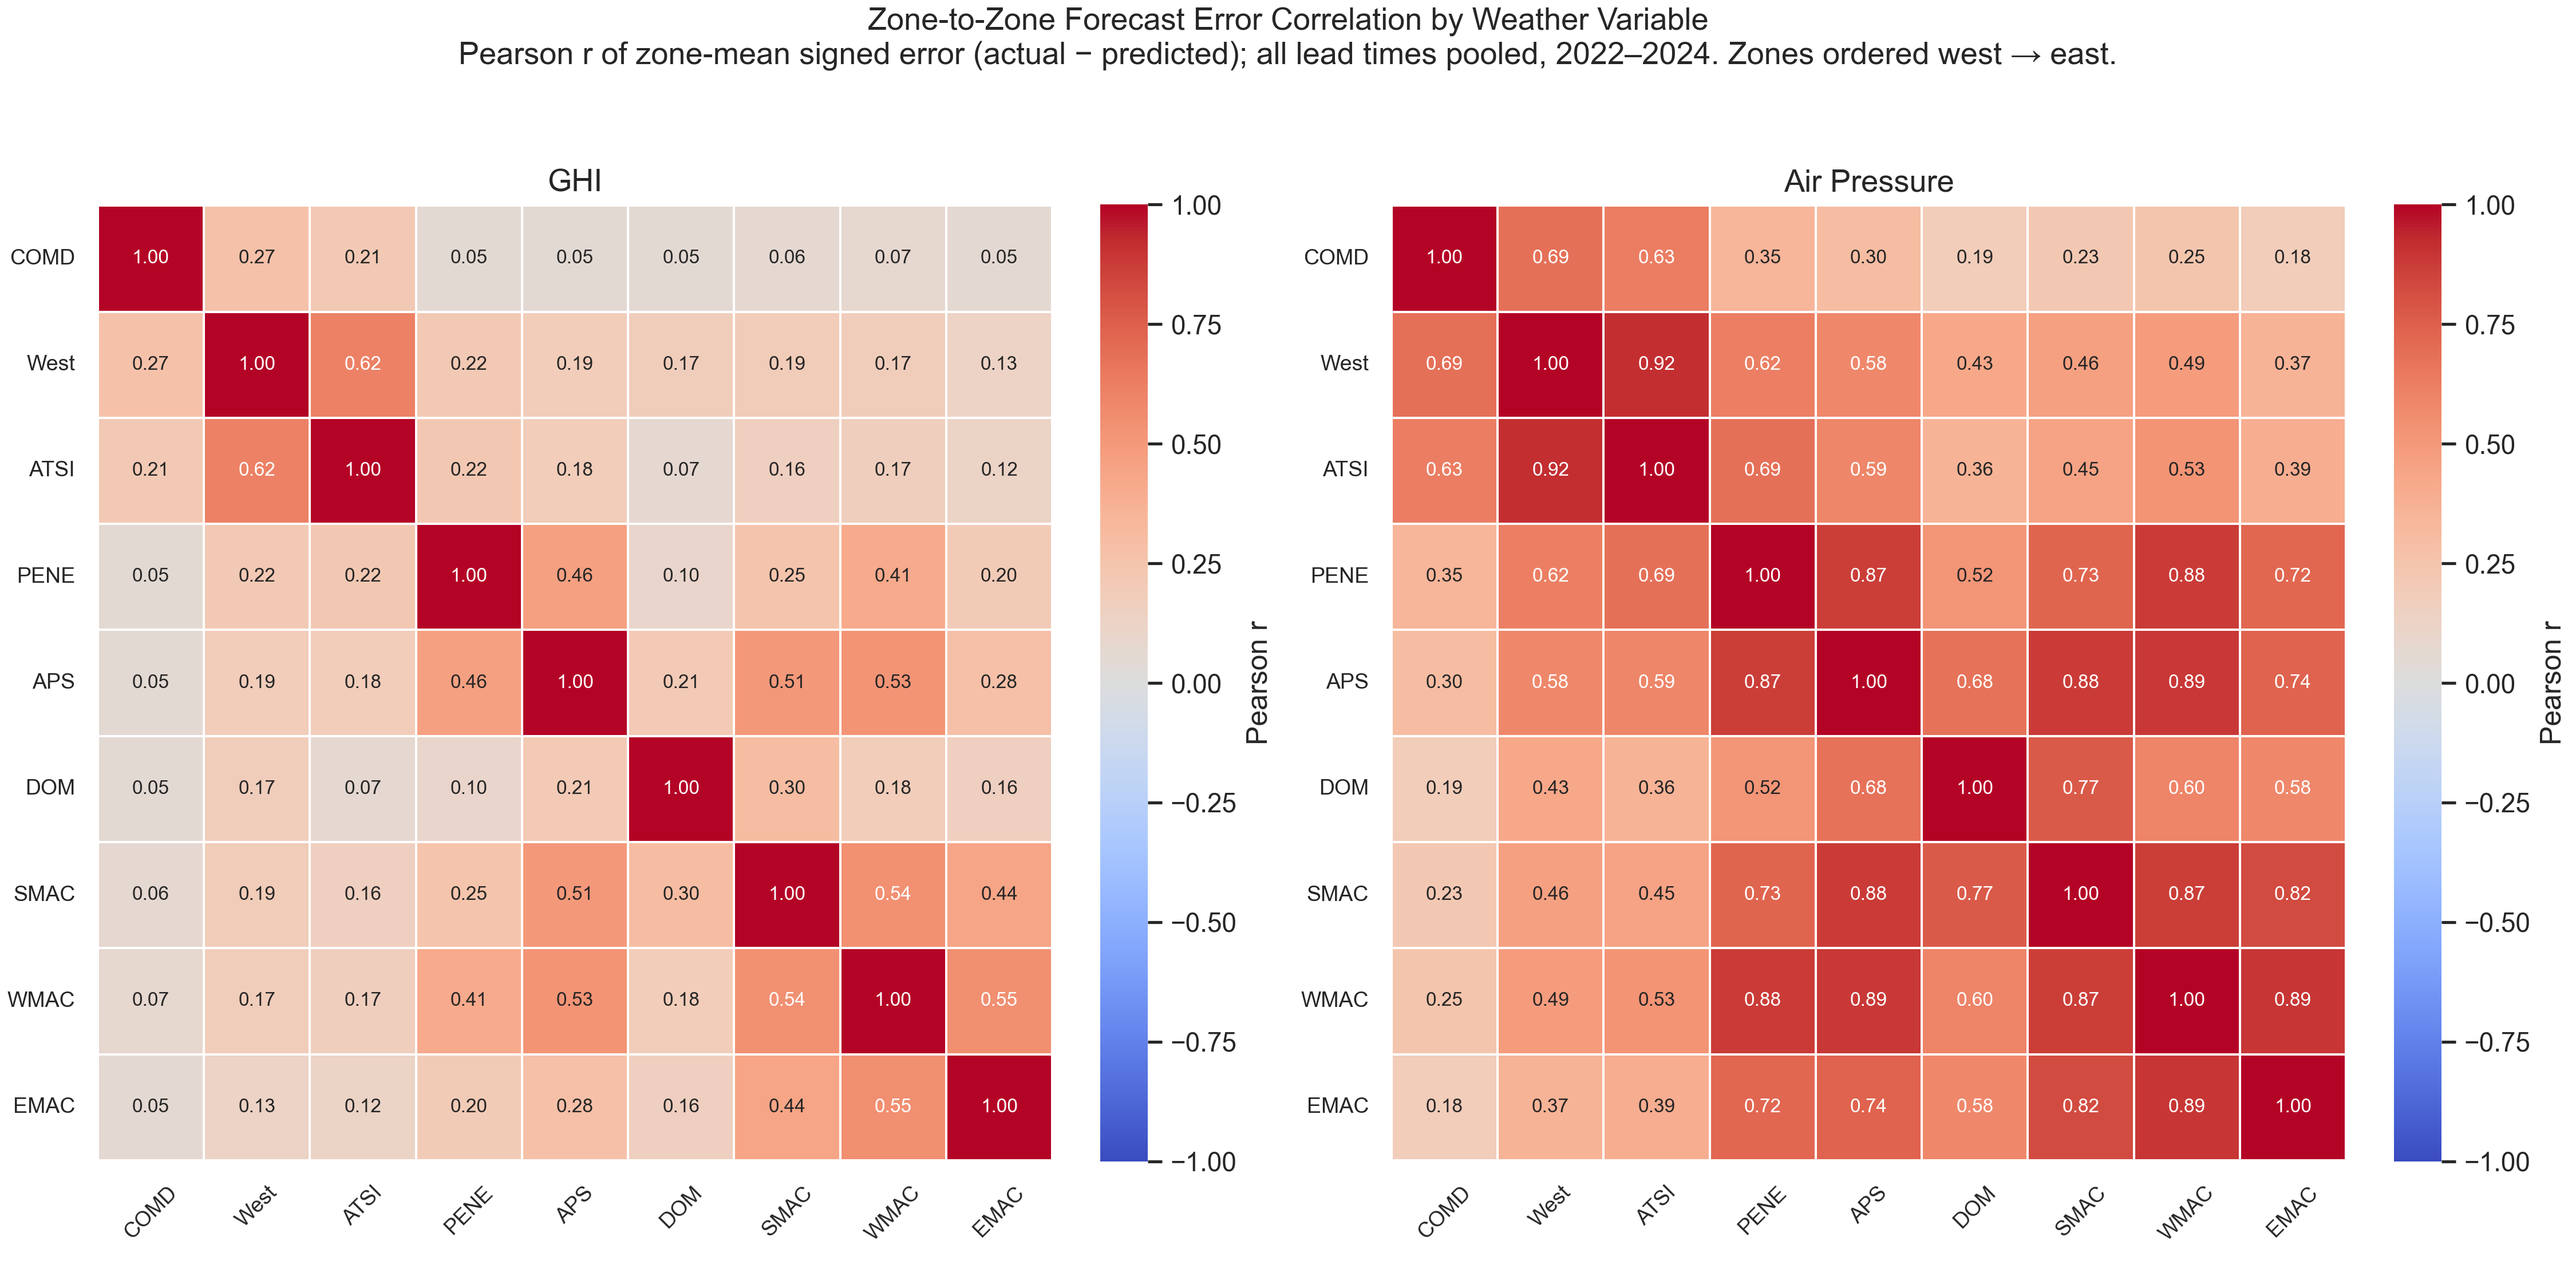
\includegraphics[width=\textwidth]{figures/Q8/embed/zone_error_correlation_ghi_pressure copy.png}
  \caption{Zone-to-zone forecast-error correlation, one $9\times 9$ matrix per variable, with
  zones ordered west~$\rightarrow$~east. Warmer off-diagonal cells indicate zones whose errors
  move together. Pressure is the warmest matrix (synoptic, regionally coherent); wind direction
  is the coolest (near-zero everywhere); GHI is also cool (local, cloud-driven). Within every
  variable the strongest correlations cluster near the diagonal, reflecting geographic adjacency.}
  \label{fig:zonecorr}
\end{figure}

Ranking variables by mean off-diagonal correlation gives, from most to least coherent:
air pressure (0.59) $>$ RH (0.56) $>$ temperature (0.41) $>$ U10 (0.27) $>$ GHI (0.24) $>$
V10 (0.22) $>$ wind speed (0.19) $>$ wind direction (0.08). Air pressure is the most spatially
coherent---neighboring zones correlate at 0.6--0.9---because pressure errors are at a synoptic scale.
GHI and wind direction are the most independent across zones.

\subsection{Spatial decay and the decorrelation length}

For a fixed lead time we compute, for every one of the $\approx \num{400000}$ site pairs, the
great-circle distance and the Pearson correlation of their signed-error series. Binning the pairs
into \SI{25}{km} distance bins and fitting an exponential
$\rho(d) = a\,e^{-d/L} + c$ yields the \emph{decorrelation length} $L$ (the e-folding distance at
which the decaying part falls to $1/e \approx 37\%$). Figure~\ref{fig:decay12} shows the headline
fit at lead~12 (solar noon).

\begin{figure}[H]
  \centering
  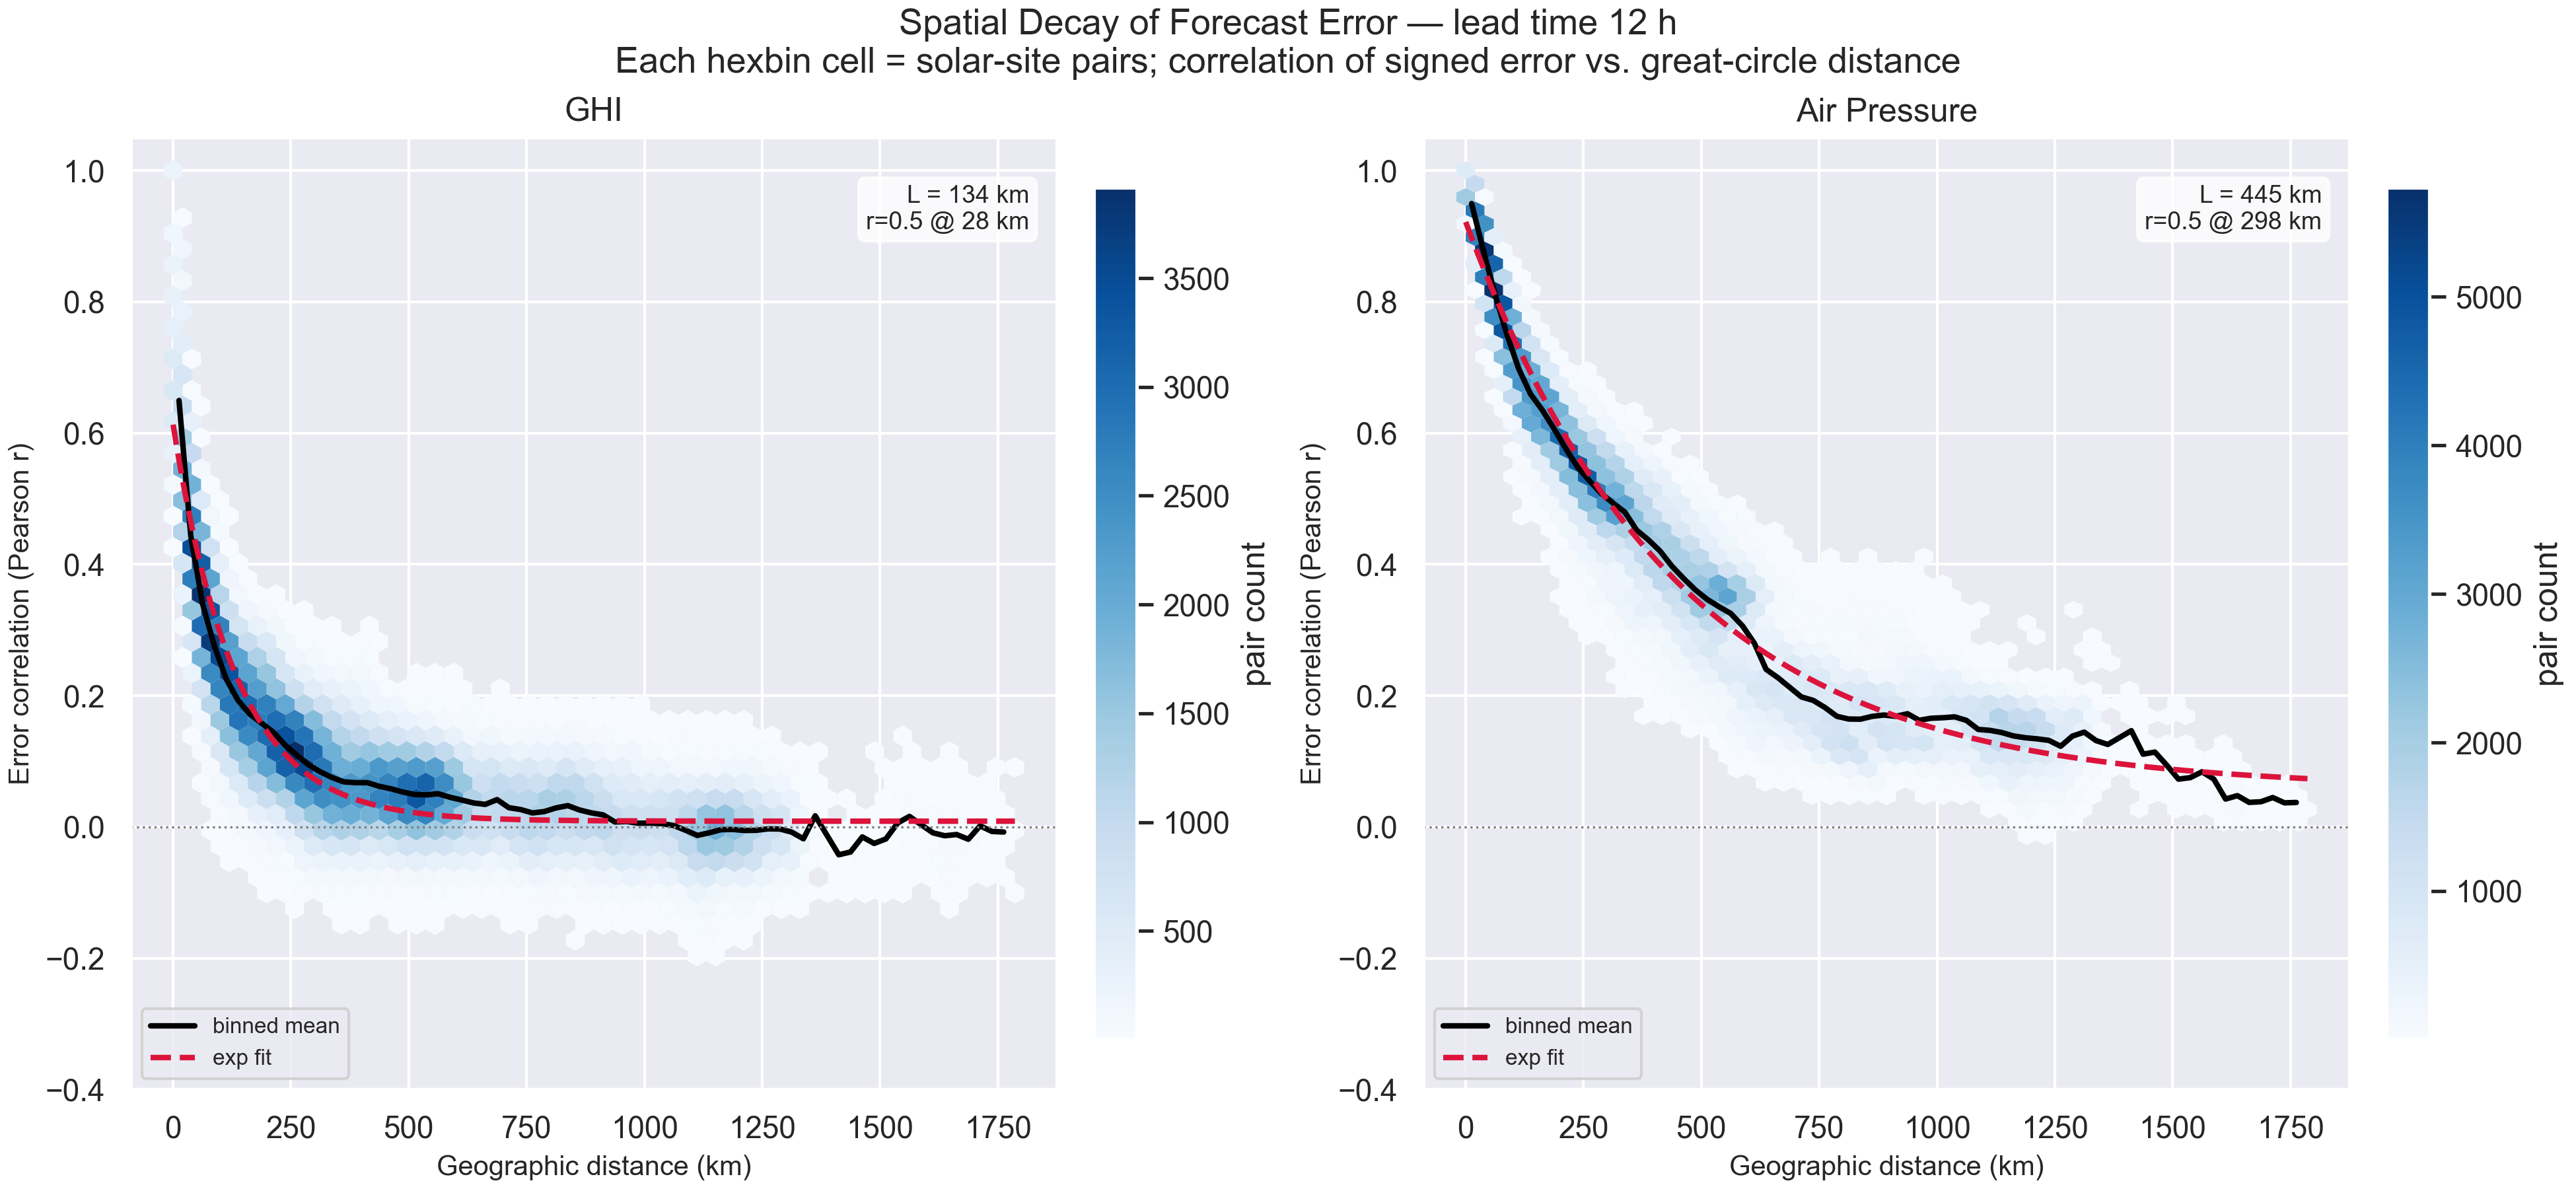
\includegraphics[width=\textwidth]{figures/Q8/embed/spatial_decay_lead12_ghi_pressure.png}
  \caption{Spatial decay of forecast error at lead~12~h (= \texttt{18z}, solar noon). Each panel
  plots error correlation versus great-circle distance for all $\approx\num{400000}$ site pairs
  (hexbin density), with the distance-binned mean (black) and fitted exponential
  $\rho(d)=a\,e^{-d/L}+c$ (crimson). Pressure is the most spatially coherent
  ($L \approx \SI{445}{km}$); temperature ($L \approx \SI{233}{km}$) and RH
  ($L \approx \SI{277}{km}$) are intermediate; GHI decorrelates fastest
  ($L \approx \SI{134}{km}$, $r=0.5$ by $\sim\SI{28}{km}$); wind direction is so noisy its fit
  never reaches $r=0.5$.}
  \label{fig:decay12}
\end{figure}

\subsection{Implications}

Forecast errors only diversify across a portfolio when sites are spaced \emph{farther apart than
$L$}. Because $L$ is shortest for GHI and wind direction, a geographically spread fleet smooths
those errors well, and that is favorable since GHI drives solar output. Pressure and
temperature errors, by contrast, stay correlated across hundreds of kilometres and barely
diversify even fleet-wide.

As lead time increases, forecast errors for most variables become spatially correlated over longer distances, so aggregating sites levels out the total error less. Thus, the portfolio gets a smaller diversification benefit because more of the fleet is wrong in the same direction at the same time. However, forecasts errors for U10 and V10 trend downward, so the errors for longer lead times are more spatially independent.

The diurnal pattern observed in U10, GHI, and wind direction indicate that time of day is a confounding variable. Data for forecasts at different initialized times is necessary to investigate this further. Regardless, this finding indicates that errors are more spatially independent during the night.
